% !TEX root =  ICRA2012-Patil.tex

We present simulation results for two scenarios: a car-like robot with second order dynamics and a nonholonomic bevel-tip flexible needle. In both scenarios, the robot moves subject to stochastic dynamics under the guidance of partial and noisy state measurements. In each case, we initialize our method with a nominal plan computed using an RRT planner \cite{Book:Lavalle06}. We empirically demonstrate that our method provides a more accurate estimation of the a priori probability distributions of the robot state and the probability of collision compared to prior methods. We also validate our method by comparing the estimated collision probability with the probability computed by Monte-Carlo simulations (considered as ground truth). We implemented our method in C++ and tested it on a 3.33 Ghz Intel\textsuperscript{\tiny \textregistered} i7\textsuperscript{\tiny TM} PC.

\subsection{Car-like Robot with Second Order Dynamics}

\begin{figure*}[!t]
{\,} \hfill
\subfigure[\label{fig:1a}]{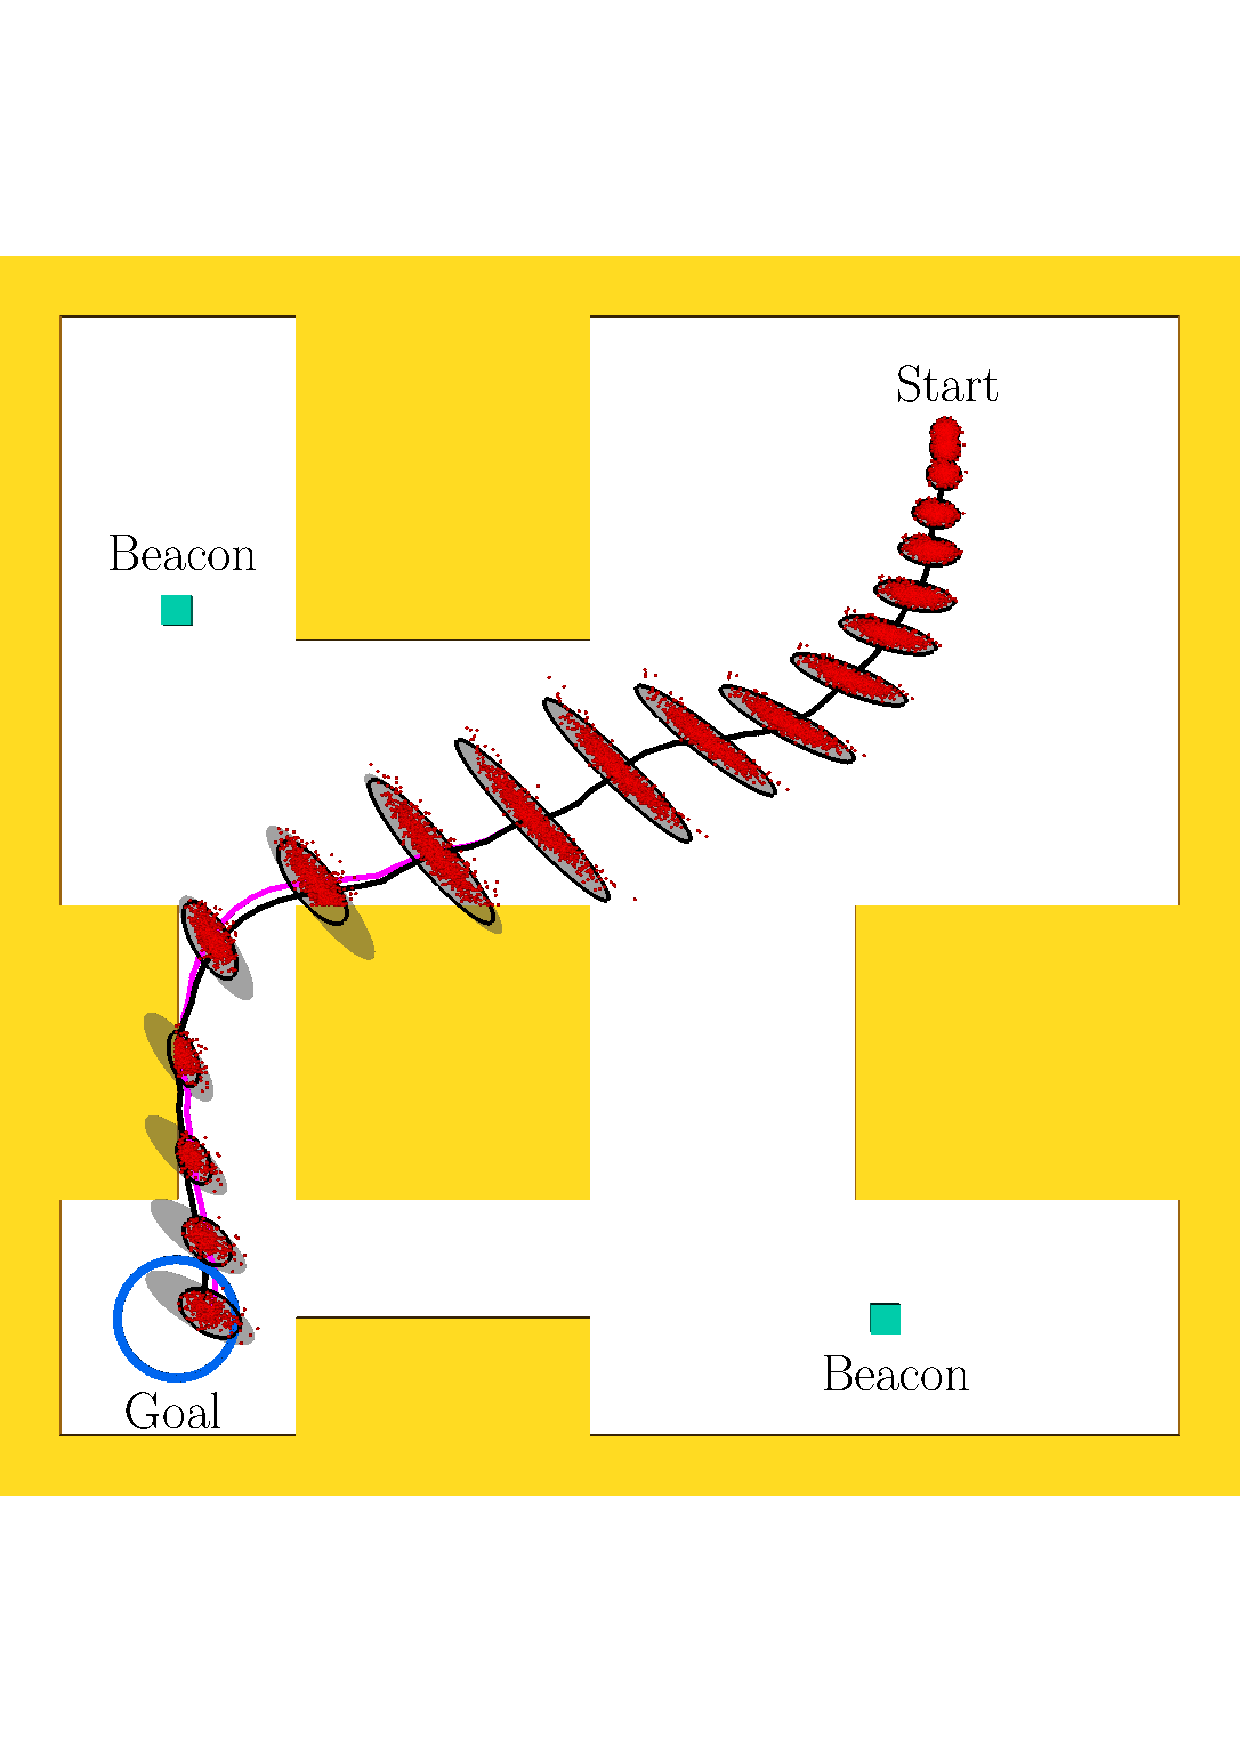
\includegraphics[width=160pt,clip]{figures/car2d/car2d-fig.pdf}}
\hfill
\subfigure[\label{fig:1b}]{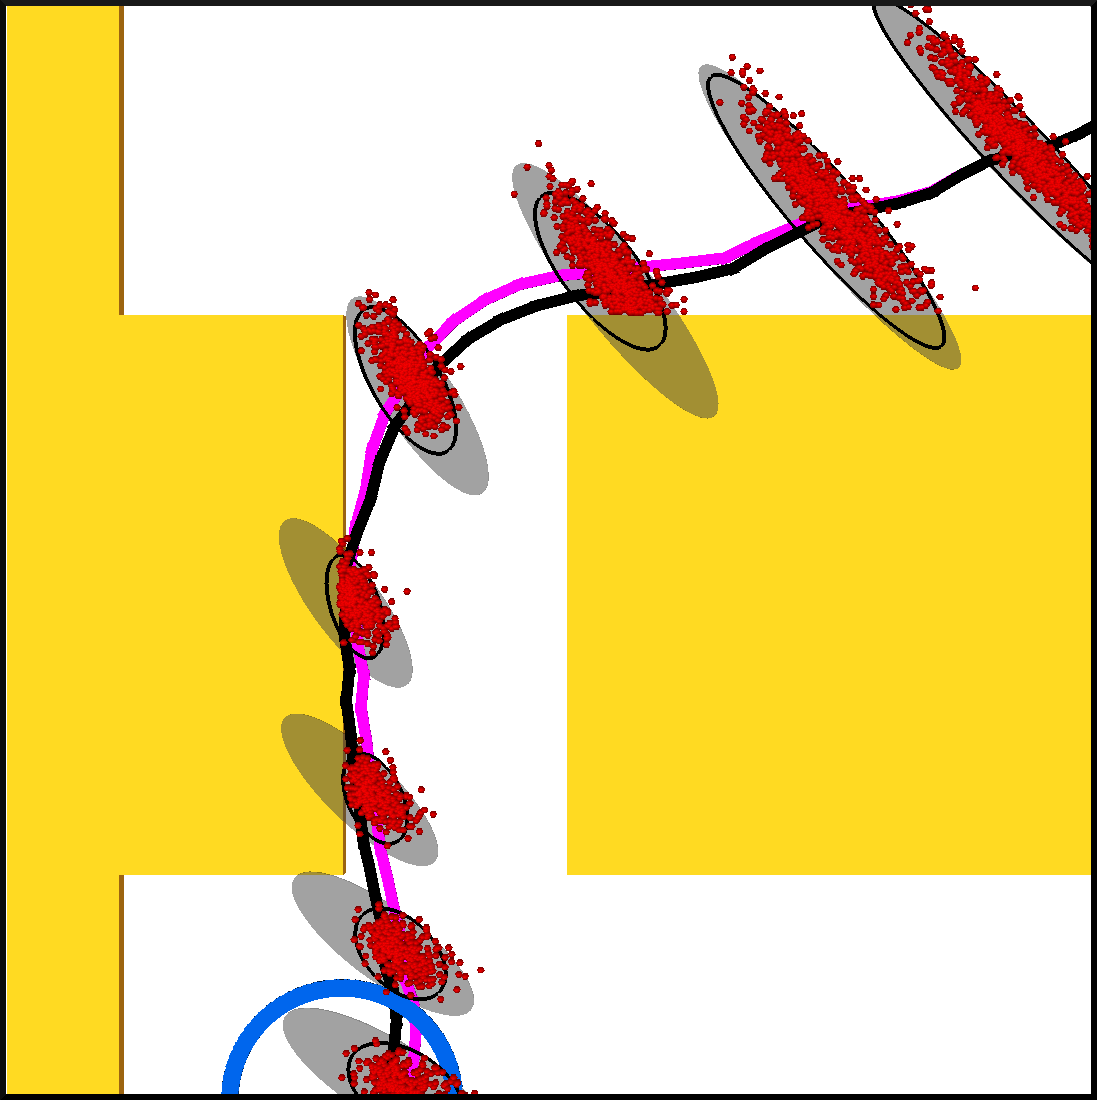
\includegraphics[width=160pt,clip]{figures/car2d/plan1-closeup.png}}
\hfill
\subfigure[\label{fig:1c}]{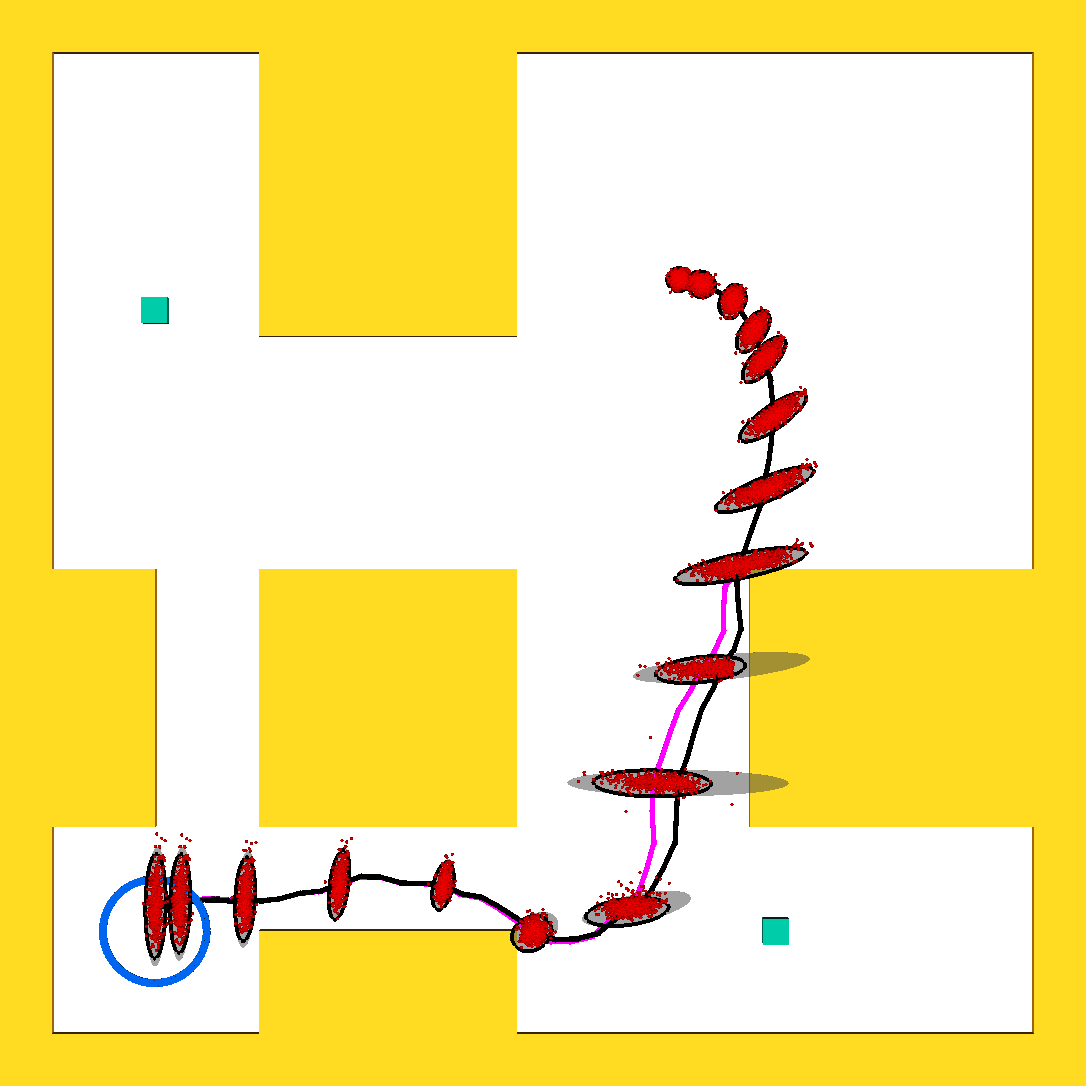
\includegraphics[width=160pt,clip]{figures/car2d/plan3.png}}
{\,} \hfill
\vspace*{-5pt}
\caption{Car-like robot with second order dynamics: (a) An initial plan (black) is computed using an RRT planner. The unconditional distributions (solid gray ellipses showing $3$ standard deviations of the Gaussian distribution) provide an overly conservative approximation of the uncertainty. Samples of the true distribution computed by Monte Carlo simulations are shown by the red dots.
Our method computes conditional distributions (black ellipses showing $3$ standard deviations), which provide an accurate estimate of the true distributions. The probability of collision estimated by our method for this example is $68.87\%$, while the probability determined by Monte-Carlo simulations is $66.26\%$. Our method provides an accurate, yet conservative, approximation of the collision probability. (b) Zoomed in view of the conditional distributions in the narrow corridor in the environment. The mean of the conditional distribution (magenta) deviates from the nominal plan due to the truncation of the distributions due to obstacle collisions. (c) Conditional and unconditional distributions computed along a second plan. The probability of collision estimated by our method for this example is $44.78\%$, while the probability determined by Monte-Carlo simulations is $42.32\%$.}
\vspace*{-15pt}
\label{fig:car2d}
\end{figure*}

We apply our method to a nonholonomic car-like robot with second order dynamics, navigating in a 2D environment with obstacles. The state of the robot, $\mathbf{x} = [x, y, \theta, v]^T \in \mathbb{R}^4$, consists of its position $[x, y]$, its orientation $\theta$, and its speed $v$. The control input $\mathbf{u} = [a, \phi]^T \in \mathbb{R}^2$, consists of the acceleration $a$, and steering angle $\phi$, corrupted by motion noise $\mathbf{m} = [\tilde{a}, \tilde{\phi}]^T \sim \mathcal{N}[\mathbf{0}, M]$. This gives the following stochastic dynamics model:
\begin{equation}
\mathbf{f}[\mathbf{x}, \mathbf{u}, \mathbf{m}] = \begin{bmatrix} x + \tau v \mathrm{cos}\theta \\ y + \tau v \mathrm{sin}\theta \\ \theta + \tau v \mathrm{tan}(\phi + \tilde{\phi})/d \\ v + \tau(a + \tilde{a}) \end{bmatrix},
\end{equation}
where $\tau$ is the time step, and $d$ is the length of the car.

The robot localizes itself using noisy signal measurements from two beacons $b_1$ and $b_2$, placed in the environment at locations $[\check{x}_1, \check{y}_1]$ and $[\check{x}_2, \check{y}_2]$ respectively. The strength of the signal decays quadratically with the distance to the beacon. The robot also measures its current speed using an on-board speedometer. The observation vector $\mathbf{z} \in \mathbb{R}^3$, consists of two readings of signal strengths from the beacons and a speed measurement from the speedometer, corrupted by sensing noise $\mathbf{n} \sim \mathcal{N}[\mathbf{0}, N]$. This gives us the following stochastic measurement model:
\begin{equation}
\mathbf{h}[\mathbf{x}, \mathbf{n}] = \begin{bmatrix} 1/((x - \check{x}_1)^2 + (y - \check{y}_1)^2 + 1) \\ 1/((x - \check{x}_2)^2 + (y - \check{y}_2)^2 + 1) \\ v \end{bmatrix} + \mathbf{n}.
\end{equation}

We consider a non-convex environment with narrow corridors to evaluate the performance of our method (Fig. \ref{fig:1a}). Fig. \ref{fig:1b} shows the discrepancy between the unconditional and conditional distributions in the presence of obstacles. The conditional distributions computed using our method provide an accurate estimate of the distribution of the collision free robot states along the plan, thus providing an accurate estimate of the probability of collision. Fig. \ref{fig:1c} shows how the mean of the conditional distribution can deviate significantly in the close vicinity of obstacles. Interestingly, the conditional and unconditional distributions become identical towards the end of the plan in the absence of obstacles.

To validate our method, we generated a set of $100$ plans using the RRT planner using randomly initialized start states. We estimated the probability of collision using our method for each of these plans. This took $0.09$ seconds. We also used a brute-force approach to estimate the ground truth probability of collision using Monte-Carlo sampling. We performed $10,000$ simulations of executions of each plan using the given controller and Kalman filter, and with artificially generated motion and measurement noise, and counted the number of collision free executions. This took $271$ seconds, which is orders of magnitude slower than our method.

Table~\ref{tab:comp} compares the collision probability estimate computed using our method with the probability computed using brute-force Monte-Carlo sampling, applying Boole's inequality to the unconditional distributions \cite{Vitus11_ICRA}, and LQG-MP \cite{vandenBerg11_IJRR}. We use the mean error as a metric to compare the probability estimates to the ground truth probability computed using sampling, across $100$ randomly generated plans.

For this example, the mean error in estimation using our method as compared to the ground truth probability is $3.0\%$. The estimate computing using our method is much more accurate than the collision quality metric provided by LQG-MP (mean error of $52.2\%$) \cite{vandenBerg11_IJRR} and the collision probability computed using the unconditional distributions directly by assuming independent probabilities (mean error of $28.0\%$) \cite{Vitus11_ICRA}, with negligible computational overhead. It is important to note that all the estimation methods, including ours, provide a conservative bound for the collision probability.

\setlength{\tabcolsep}{1.5pt}
\begin{table}[htb]
\centering
        \resizebox{3.4in}{!}{
        \begin{tabular}{|c||c||c|c||c|c||c|c|}
                \hline
                Robot & Sampling & \multicolumn{2}{|c||}{Our method} &\multicolumn{2}{|c||}{Unconditional}   &\multicolumn{2}{|c|}{LQG-MP} \\
                \hline
                & Time       &MAE      &Time   &MAE        &Time   &MAE      &Time\\
                & (secs)     &prob(\%) &(secs) &prob(\%)   &(secs) &prob(\%) &(secs)\\
                \hline
                %& & & & & & &\\
                car & 271 & 3.0 & 0.09 & 28.0 & 0.06 & 52.2 & 0.04 \\
                & &($\pm$ 1.9) & &($\pm$ 15.1) & &($\pm$ 15.4) &\\
                \hline
                %& & & & & & &\\
                needle & 388 & 5.0 & 1.4 & 20.7 & 1.2 & 61.7 & 1.0\\
                & & ($\pm$ 3.0)& & ($\pm$ 6.9) & & ($\pm$ 11.5) &\\
                \hline
        \end{tabular}
        }
        \caption{Comparison of our method with existing approaches over $100$ randomly generated plans in terms of mean error from ground truth probability estimated by sampling.}
        \label{tab:comp}
\vspace{-15pt}
\end{table}

\subsection{Nonholonomic Bevel-tip Flexible Needle}

\begin{figure*}[!t]
{\,} \hfill
%\subfigure[\label{fig:2a}]{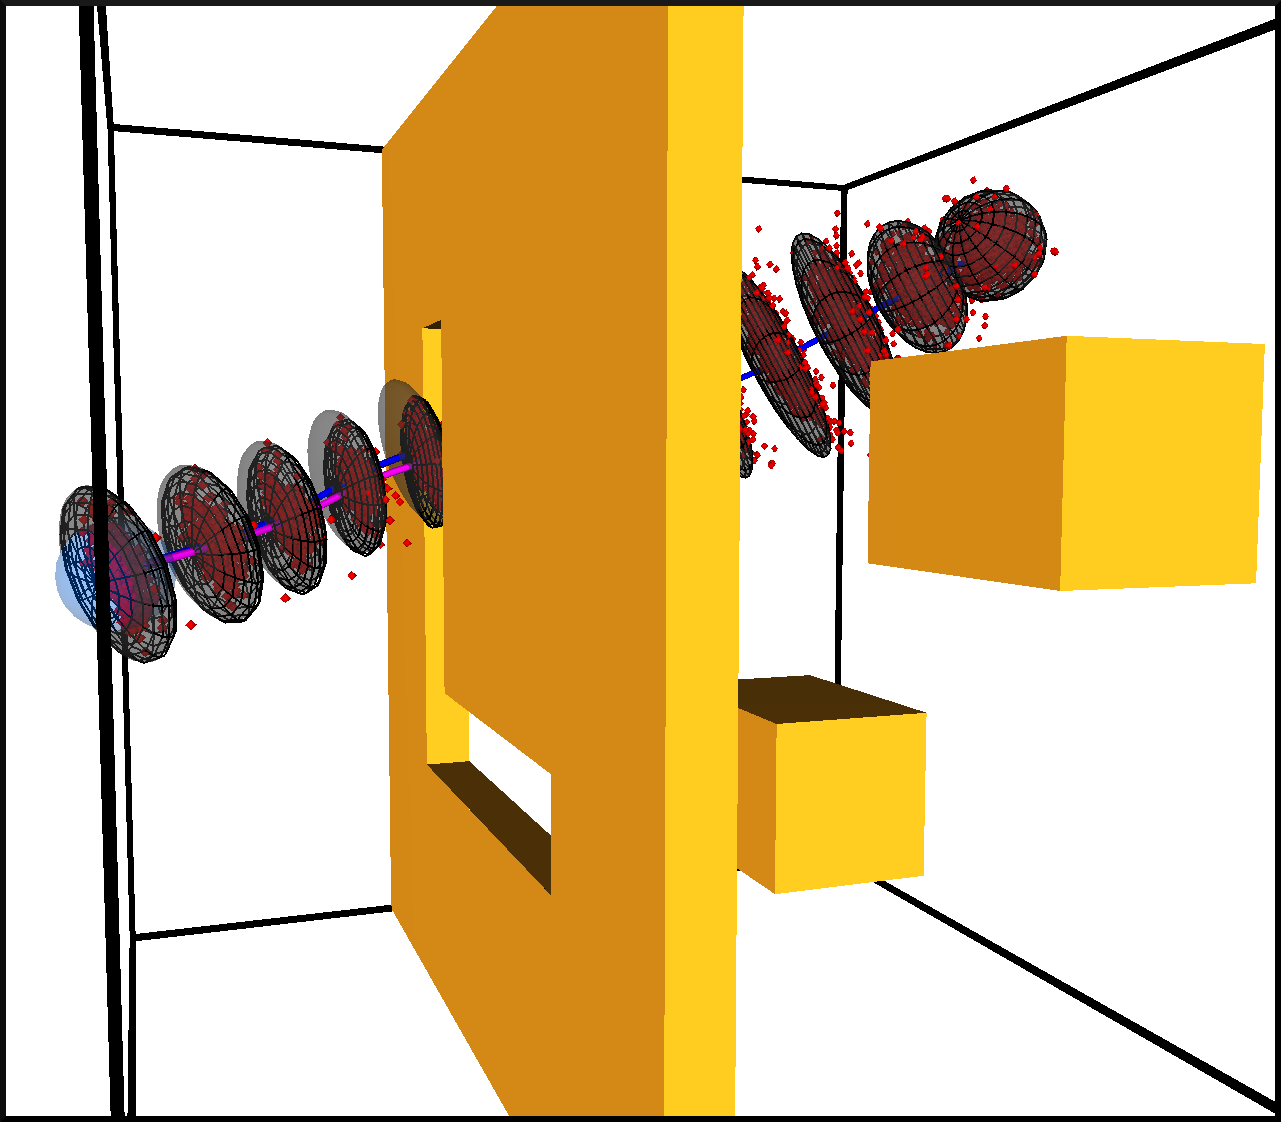
\includegraphics[width=160pt,clip]{figures/needle3d/plan1.png}}
\subfigure[\label{fig:2a}]{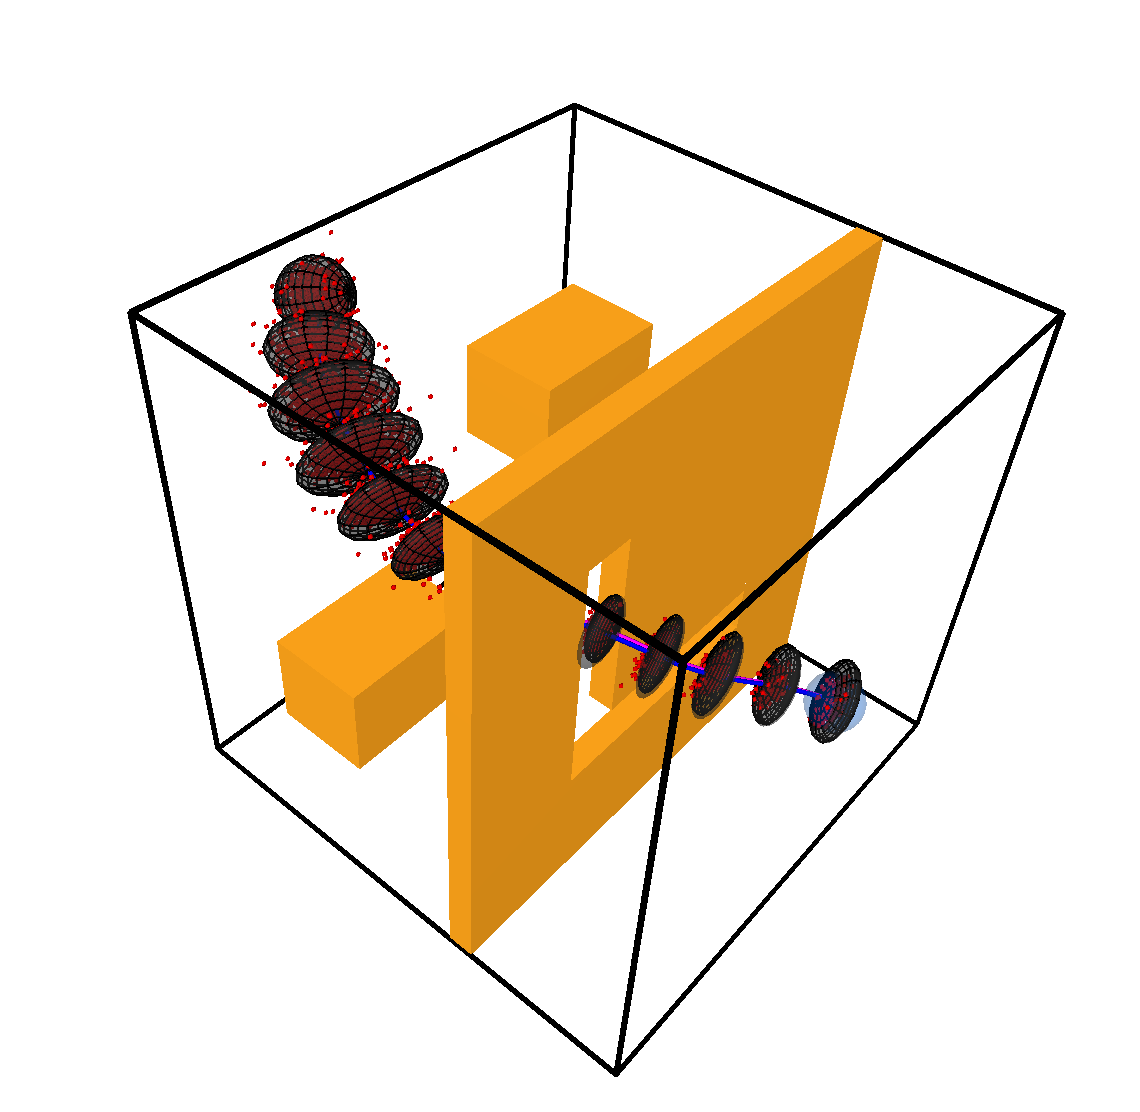
\includegraphics[trim=0pt 30pt 0pt 0pt, clip, width=160pt,clip]{figures/needle3d/plan1-top.png}}
\hfill
\subfigure[\label{fig:2b}]{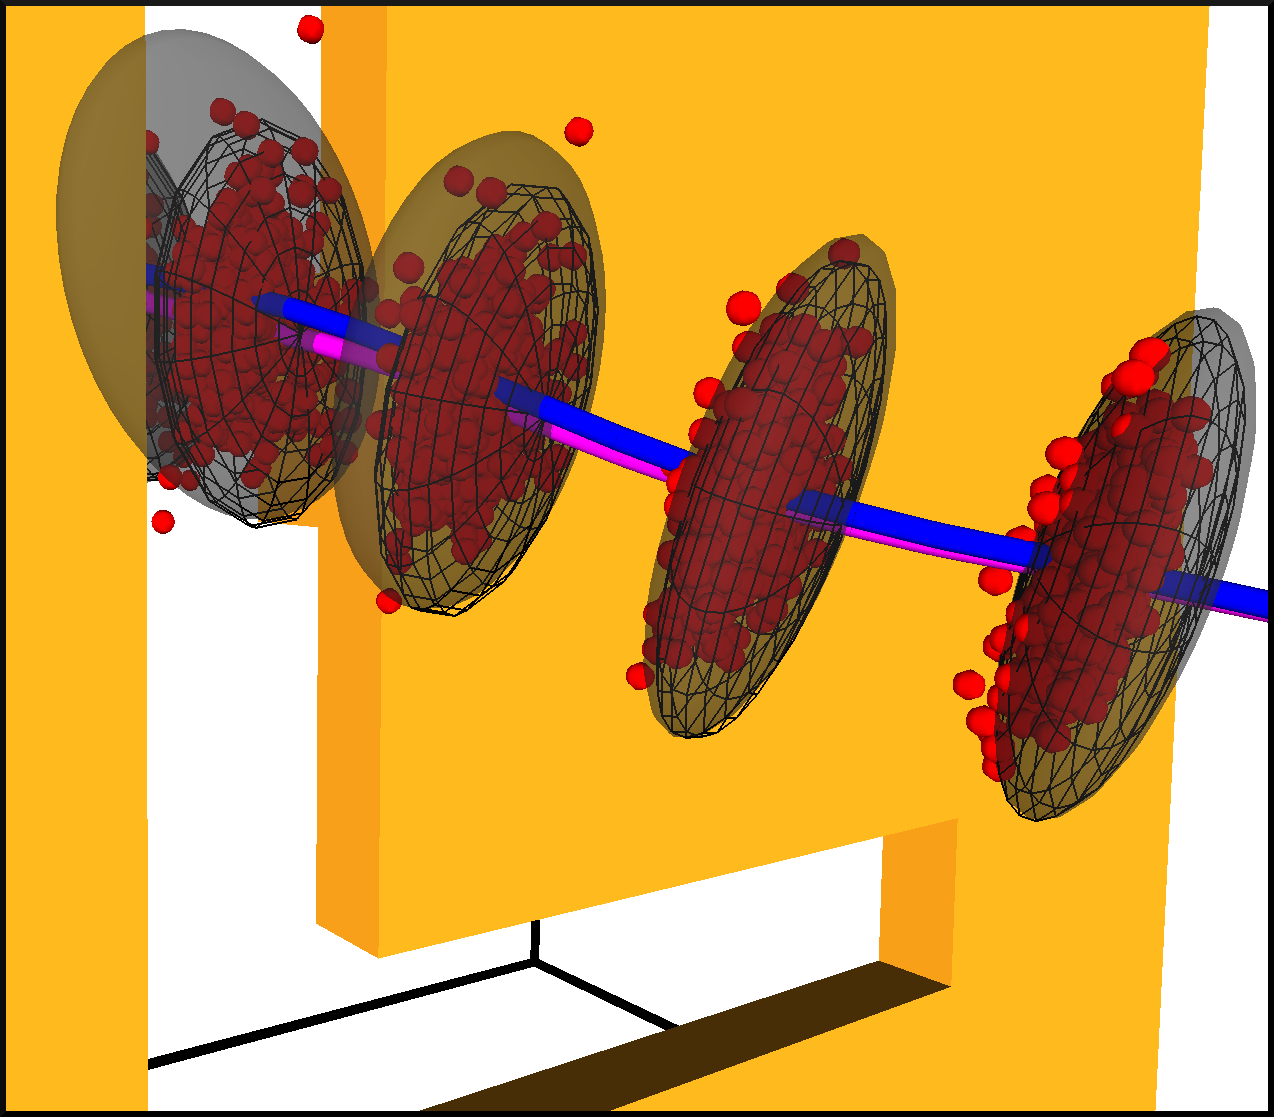
\includegraphics[width=160pt,clip]{figures/needle3d/plan1-closeup.png}}
\hfill
\subfigure[\label{fig:2c}]{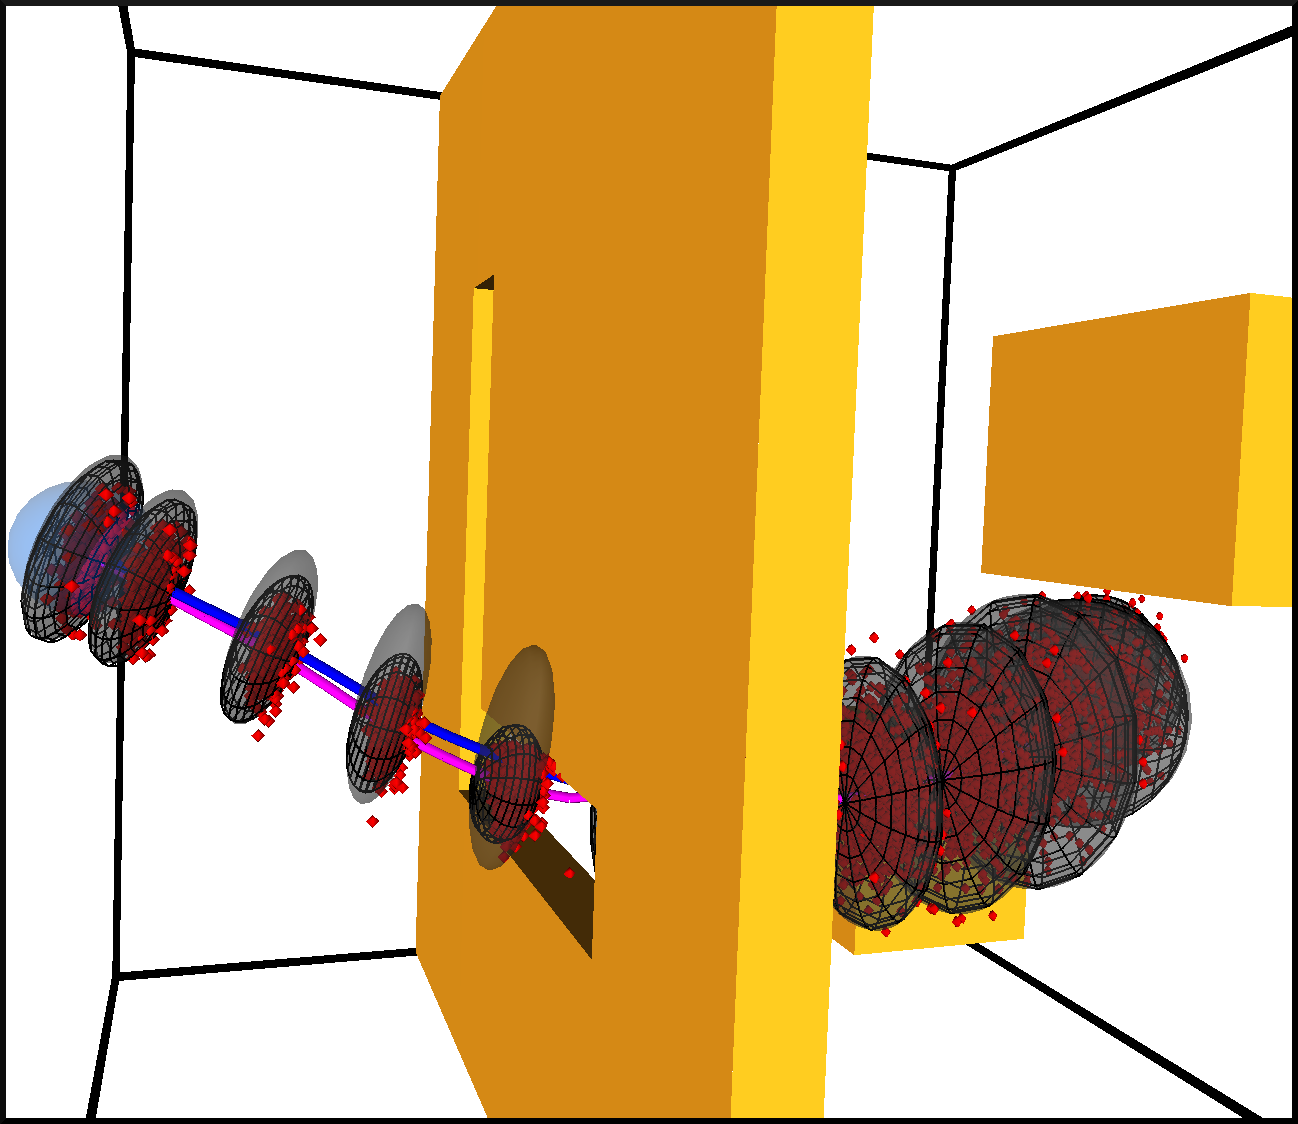
\includegraphics[width=160pt,clip]{figures/needle3d/plan2.png}}
{\,} \hfill
\vspace*{-5pt}
\caption{Nonholonomic bevel-tip steerable needle: (a) The unconditional distributions (solid gray ellipsoids, $3$ standard deviations) provide an overly conservative approximation of the uncertainty. Our method computes conditional distributions (black wireframe ellipsoids, $3$ standard deviations), which provide an accurate estimate of the probability distributions of the feasible robot states (shown in red). The probability of collision estimated by our method for the given plan is $54.5\%$, while the probability determined by Monte-Carlo simulations is $50.4\%$. Our method provides an accurate, yet conservative approximation of the collision probability. (b) Zoomed in view of the conditional distributions in the narrow corridor in the environment. The mean of the conditional distribution (magenta) deviates from the nominal plan due to the truncation. (c) The probability of collision estimated by our method for a second plan is $43.9\%$, while the probability determined by Monte-Carlo simulations is $42.2\%$.}
\vspace*{-15pt}
\label{fig:needle3d}
\end{figure*}

We also apply our method to a nonholonomic bevel-tip flexible needle \cite{Cowan2011_Chapter}, navigating in a 3D environment with obstacles. This class of needles offers improved mobility,
enabling needles to reach previously inaccessible targets while maneuvering around sensitive or impenetrable areas.

The state of the needle $\mathbf{x}$, is described by the $4 \times 4$ matrix $X = \left[\begin{smallmatrix} R & \mathbf{p} \\ \mathbf{0} & 1 \end{smallmatrix} \right] \in SE(3)$, where $\mathbf{p} \in \mathbb{R}^3$ is the position of the needle tip, and $R \in SO(3)$ is the rotation matrix that encodes the orientation of the needle tip, relative to a world coordinate frame. The needle naturally moves along constant curvature paths when inserted into tissue, but the curvature of the needle motion can be varied by duty cycled spinning of the needle during insertion. Under these modeling assumptions \cite{vandenBerg10_WAFR}, the control input $\mathbf{u} = [v, w, \kappa]^T \in \mathbb{R}^3$, consists of the insertion speed $v$, rotation speed applied at the base of the needle $w$, and the curvature $\kappa$.

It is convenient to describe the dynamics of the needle tip in terms of the instantaneous twist $U \in se(3)$ expressed in a local coordinate frame attached to the needle tip, given by:
\begin{equation}
U = \begin{bmatrix} [\mathbf{w}] & \mathbf{v} \\ \mathbf{0} & 0 \end{bmatrix}, ~ \mathbf{w} = \begin{bmatrix} v\kappa & 0 & w \end{bmatrix}^T, ~ \mathbf{v} = \begin{bmatrix} 0 & 0 & v \end{bmatrix}^T,
\end{equation}
where the notation $[\mathbf{s}]$ for a vector $\mathbf{s} \in \mathbb{R}^3$ refers to the $3 \times 3$ skew-symmetric cross-product matrix. The instantaneous twist $\tilde{U}$ that encodes the additive motion noise $\mathbf{m} = [\tilde{\mathbf{v}} ~ \tilde{\mathbf{w}}]^T \sim  \mathcal{N}[\mathbf{0}, M]$, can be similarly expressed.

Given a time step $\tau$, the stochastic discrete-time dynamics of the needle-tip is given by the following model:
\begin{equation}
\mathbf{f}[\mathbf{x}, \mathbf{u}, \mathbf{m}] = X\mathrm{exp}(\tau (U + \tilde{U})).
\end{equation}

We also assume that we receive partial, noisy feedback on only the position of the needle tip $\mathbf{p}$, and not its orientation. This is a reasonable assumption since current medical imaging
technologies such as ultrasound do not allow for measuring the full state of the needle tip (as the imaging resolution is often too low to infer its orientation). The noise in the
sensor measurement is modeled as $\mathbf{n} \sim \mathcal{N}[\mathbf{0}, N]$. This gives the following stochastic measurement model:
\begin{equation}
\mathbf{h}[\mathbf{x}, \mathbf{n}] = \mathbf{p} + \mathbf{n}.
\end{equation}
We follow the approach suggested in \cite{vandenBerg10_WAFR} to approximate the given nonlinear dynamics and measurement models with local linearizations around the nominal plan.

We consider a non-convex environment with a L-shaped narrow corridor and other obstacles to evaluate the performance of our method (Fig. \ref{fig:2a}). Fig. \ref{fig:2b} shows the discrepancy between the unconditional and conditional distributions in the presence of obstacles. The conditional distributions computed using our method provide an accurate estimate of the distribution of the collision free robot states along the plan, thus providing an accurate estimate of the probability of collision.

Similar to the analysis performed for the previous example, we generated a set of $100$ plans using the RRT planner starting from the goal state. We estimated the probability of collision using our method for each of these plans. This took $1.4$ seconds. We also used a brute-force approach to estimate the ground truth probability of collision using Monte-Carlo sampling. We performed $10,000$ simulations of executions of each plan with artificially generated motion and measurement noise, and counted the number of collision free executions. This took $388$ seconds, which is orders of magnitude slower than our method.

Table \ref{tab:comp} shows the results of how our method compares to the ground truth and prior approaches. For the given example, the mean error in estimation using our method as compared to the ground truth probability is $5.0\%$. The estimate computed using our method is much more accurate than the collision quality metric provided by LQG-MP (MAE $61.7\%$) \cite{vandenBerg11_IJRR} and the collision probability computed using the unconditional distributions directly by assuming independent probabilities (MAE $20.7\%$) \cite{Vitus11_ICRA}, while incurring negligible computational overhead. 